\chapter{Практическое применение}
В качестве доказательства применимости разрабатываемой, в рамках данной работы, группы ассетов была проведена интеграция в проект виртуальной био-технологической лаборатории DML BioLab. Было осуществлено портирование кодовой базы ATF с версии движка Unity 2019.3.6f1 на версию Unity 2017.3.1f1. 

Был создан тест, успешное прохождение которого и завершало бы доказательство. Критерием успешности прохождения данного теста являлся задокументированный в виде видеофайла факт успешной записи и прохождения первого шага в первом сценарии DML BioLab.

Первый шаг в выбранном сценарии составляет следующую группу действий: Взятие баночки PBS+20Tween (буферного раствора) и заполнение её содержимым ванночки для набора, с помощью диспенсеров (многоканальных или одноканальных капиллярных заборных устройств для жидкостей). 

\section{Портирование на Unity 2017.3.1f1}
Первая стадия портирования состоит в подготовке проекта DML BioLab к импортированию, а именно создаётся резервная копия проекта, которая отделяется от системы контроля версий  Perforce.

Так как исходный код ATF написан с использованием .NET Framework 4.6 и версией языка CSharp 7.0, а исходный код проекта виртуальной лаборатории DML BioLab написан на .NET Framework 3.5 Stable и версией языка 6.0, необходимо было перевести все тела методов и параметров перехватчика с тел лямбда-выражений, на обыкновенные блоки (см. пример в приложении \ref{atf_methods_refactor_example}).

В то же время, перевод с версии .NET фремворка 3.5 на 4.6 не составил труда, и был осуществлён путём изменения соответствующей конфигурации (см. рисунок \ref{player_conf}) Player в Unity Editor.

\begin{figure}[H]
	\centering
	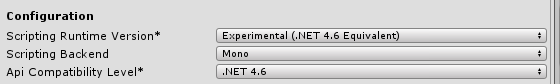
\includegraphics[width=\linewidth]{player_config.png}
	\caption{Конфигурация среды исполнения Player}
	\label{player_conf}
\end{figure}

\section{Интеграция в симулятор VRTK}
Проект виртуальной био-технологической лаборатории, в качестве менеджера VR устройств (контроллеров и шлема), использует фреймворк VRTK \cite{vrtk}. В процессе разработки приложения с использованием данного фреймворка, можно обойтись и без настоящего VR устройства, используя встроенный его симулятор, который автоматически заменяется на реальное VR устройство при его доступности. Однако стоит заметить, что если не использовать симулятор, то в качестве метода взятия ввода используется система интерфейсов-маркеров, что не покрывается разработанным перехватчиком.

Данный симулятор использует в качестве устройств ввода клавиатуру и мышку, а в качестве метода взятия ввода -- комбинацию из Input и BaseInput классов. Описанная комбинация позволяет выполнить автоматическую интеграцию группы ассетов ATF. 

Далее выясняется, что некоторые из методов класса Input по взятию ввода не присутствуют в классе BaseInput в статичной или в объектной доступности. Так как класс Input является sealed (недоступен для наследования) и в языке CSharp невозможно множественное наследование классов, а для полноценной работы перехватчика необходимо было использовать методы одновременно из классов Input, BaseInput и MonoSingleton<ATFInput>, было принято решение использовать структурный паттерн Simulated Multiple Inheritance (SMI) (см. рисунок \ref{smi_diagram}).

\begin{figure}[H]
	\centering
	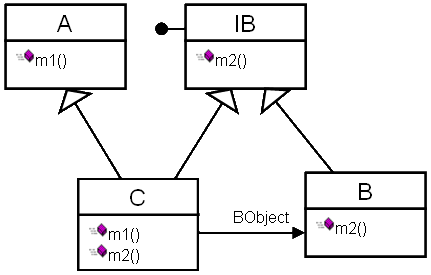
\includegraphics[width=0.6\linewidth]{multiinheritance.png}
	\caption{Диаграмма классов для паттерна SMI}
	\label{smi_diagram}
\end{figure}

В качестве А класса на рисунке \ref{smi_diagram} используется класс MonoSingleton<AtfInput>, в качестве IB взят IBaseInput интерфейс, который объединяет интерфейсы BaseInput класса и Input класса, а C класс является классом-арбитром AtfInput. Экземпляр класса BaseInput загружается в память на этапе инъекции зависимостей. Данное нововведение позволяет обращаться ко всем, включая объектные методы, по параметру AtfInput.Instance, в то же время все статичные методы остались по-умолчанию доступны по ссылке на класс AtfInput.

Необходимость создания статического и объектного доступа к методам перехватчика была продиктована именно вышеописанной проблемой.

В результате интеграции был успешно проведён тест, результаты которого находятся в открытом доступе на сайте YouTube.com \cite{video}.